% Cronograma de pesquisa (gráfico de Gantt)
% Feito para o ÉguaTeX (eguatex.com.br). Uso livre (CC0 1.0).
%
% Compile e pronto: sai só a figura, em PDF.
% Para pôr no seu trabalho, use o PDF com \includegraphics ou copie
% o bloco tikzpicture para dentro de uma figure.
\documentclass[tikz,border=4pt]{standalone}
\usepackage[T1]{fontenc}
\usepackage{lmodern}

\colorlet{corBarra}{blue!55!black}

\begin{document}
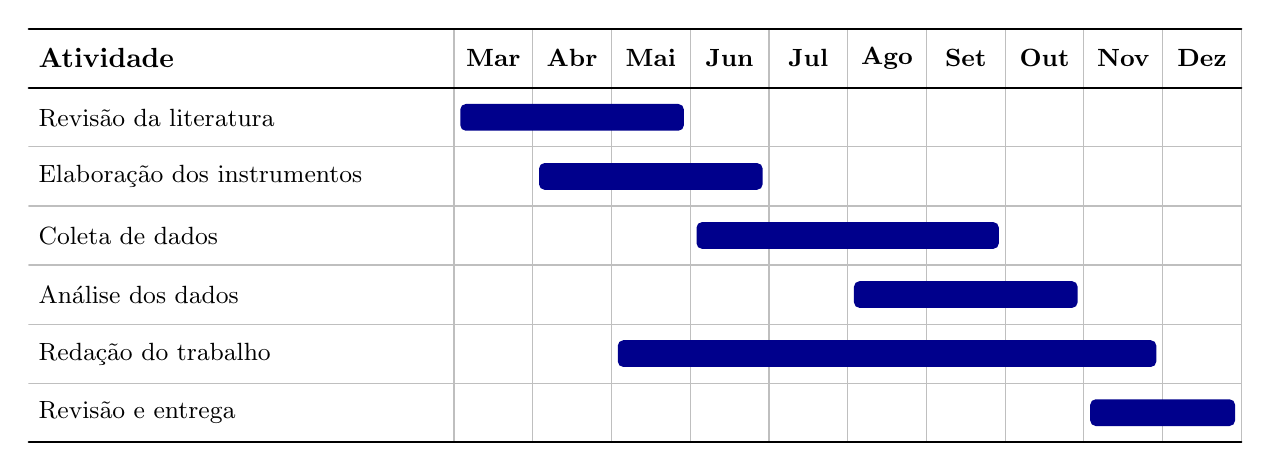
\begin{tikzpicture}[line cap=round, line join=round]

% Mude os meses e as atividades aqui.
% Atividade: nome/primeiro mês/último mês, contando os meses a partir de 1.
\def\meses{Mar,Abr,Mai,Jun,Jul,Ago,Set,Out,Nov,Dez}
\def\atividades{
  Revisão da literatura/1/3,
  Elaboração dos instrumentos/2/4,
  Coleta de dados/4/7,
  Análise dos dados/6/8,
  Redação do trabalho/3/9,
  Revisão e entrega/9/10}
\def\coluna{1}     % largura de cada mês, em cm
\def\linha{0.75}   % altura de cada linha, em cm
\def\nomes{5.4}    % largura da coluna das atividades, em cm

% conta meses e atividades
\foreach \m [count=\n] in \meses {\xdef\nm{\n}}
\foreach \a [count=\n] in \atividades {\xdef\na{\n}}

% cabeçalho
\node[anchor=west, font=\bfseries] at (0,{\linha/2}) {Atividade};
\foreach \m [count=\j] in \meses
  \node[font=\bfseries\small] at ({\nomes+(\j-0.5)*\coluna},{\linha/2}) {\m};

% grade
\foreach \j in {0,...,\nm}
  \draw[black!25] ({\nomes+\j*\coluna},\linha) -- ({\nomes+\j*\coluna},{-\na*\linha});
\foreach \i in {1,...,\na}
  \draw[black!25] (0,{-\i*\linha}) -- ({\nomes+\nm*\coluna},{-\i*\linha});
\draw[line width=0.8pt] (0,0) -- ({\nomes+\nm*\coluna},0);
\draw[line width=0.8pt] (0,\linha) -- ({\nomes+\nm*\coluna},\linha);
\draw[line width=0.8pt] (0,{-\na*\linha}) -- ({\nomes+\nm*\coluna},{-\na*\linha});

% atividades e barras
\foreach \nome/\ini/\fim [count=\i] in \atividades {
  \node[anchor=west, font=\small] at (0,{-(\i-0.5)*\linha}) {\nome};
  \fill[corBarra, rounded corners=2pt]
    ({\nomes+(\ini-1)*\coluna+0.08},{-(\i-0.5)*\linha-0.17})
    rectangle ({\nomes+\fim*\coluna-0.08},{-(\i-0.5)*\linha+0.17});
}
\end{tikzpicture}
\end{document}
